\chapter{RAG (Retrieval-Augmented Generation)}
\pagestyle{fancy}\lhead{\textbf \footnotesize\it{RAG (Retrieval-Augmented Generation}}
\pagestyle{fancy}\chead{} \pagestyle{fancy}\rhead{}
\pagestyle{fancy}\lfoot{\textbf {\small\it{Univ-Mascara/Computer Science: 2025}}} 
\pagestyle{fancy}\cfoot{} \pagestyle{fancy}\rfoot{\thepage}
%%%%%%%%%%%%%%%%%%%%%%%%%%%%%%%%%%%%%%%%
\section{ Introduction}\label{start2}

Large language models (LLMs) have seen significant advancements but face challenges, particularly in tasks that demand extensive knowledge or deal with queries beyond their training data. These limitations often result in inaccuracies or “hallucinations.” To address this, Retrieval-Augmented Generation (RAG) supplements LLMs by retrieving relevant document chunks from external knowledge sources based on semantic similarity. By doing so, RAG helps reduce factual errors, allowing LLMs to produce more accurate content. This has led to the widespread adoption of RAG, particularly in chatbots and other real-world applications, making it a crucial technology in advancing the capabilities of LLMs.
\section{Fundamentals of Retrieval-Augmented Generation}
RAG represents a significant advancement in the capabilities of large language models (LLMs) by integrating external knowledge retrieval with the generation of text. Understanding the individual components of retrieval and generation is essential to appreciate how their synergy improves the overall performance of RAG systems.
\subsection{Definition of (RAG)}
Retrieval-Augmented Generation (RAG) is a technique that leverages the strengths of pre-trained large language models (LLMs) and external data sources. By merging the generative abilities of LLMs like GPT-3 or GPT-4 with the accuracy of specialized data search mechanisms, RAG systems can generate more sophisticated and contextually relevant responses\cite{selvaraj2024}.
\subsection{Historical Development of (RAG)}
The foundations of Retrieval-Augmented Generation (RAG) can be traced back to traditional information retrieval (IR) systems,  Early models primarily relied on keyword matching and simple ranking mechanisms to retrieve relevant documents from databases, establishing a basic framework for information access. The landscape began to shift with the rise of neural networks in the 2010s. Notable innovations like Word2Vec and Transformer-based architectures enabled retrieval methods to incorporate deeper semantic understanding, paving the way for more sophisticated document retrieval processes.
A significant advancement occurred with the introduction of dense passage retrieval (DPR) in 2020, which utilized bi-encoder architectures to map both queries and documents into dense vector spaces. 
The integration of these advanced retrieval techniques with large language models (LLMs) became a focal point as models like GPT-3 gained prominence. Researchers explored how LLMs could be augmented with retrieval capabilities, leading to the development of RAG systems that leverage the strengths of both retrieval and generative capabilities\cite{gao2024retrieval}.
\subsection{Differences between (RAG), fine-tuning and transfer learning}
Recent advances in natural language processing have led to the development of three prominent methodologies for enhancing language models: Retrieval-Augmented Generation (RAG), fine-tuning, and transfer learning.

RAG, as described by Lewis et al. \cite{lewis2020retrieval}, integrates external retrieval mechanisms with generative models. This approach enables the model to dynamically access and incorporate relevant information from external knowledge bases during the generation process, thereby addressing limitations in its internal memory and providing more accurate responses for knowledge-intensive tasks.

Fine-tuning, detailed by Howard and Ruder \cite{howard2018universal}, involves adapting a pre-trained model to a specific task by further training it on a targeted dataset. This process refines the model’s parameters to better capture the nuances of the task at hand, leading to improved performance even when the available domain-specific data is relatively limited.

Transfer learning, as exemplified by Devlin et al. \cite{devlin2018bert}, refers to the broader strategy of leveraging a model that has been pre-trained on large, diverse datasets for use in various downstream tasks. This method capitalizes on the rich, generalized representations learned during the pre-training phase, and then applies task-specific adaptations to achieve state-of-the-art results across a range of applications.

Collectively, these methodologies offer complementary strategies to enhance language model performance, each contributing unique advantages and addressing different challenges in the field of natural language processing.

\section{Types of (RAG) Systems}
As detailed in \cite{gao2024retrieval}, the evolution of Retrieval-Augmented Generation (RAG) can be categorized into three distinct phases: Naive RAG, Advanced RAG, and Modular RAG .
\begin{figure}[h]
	\centering
	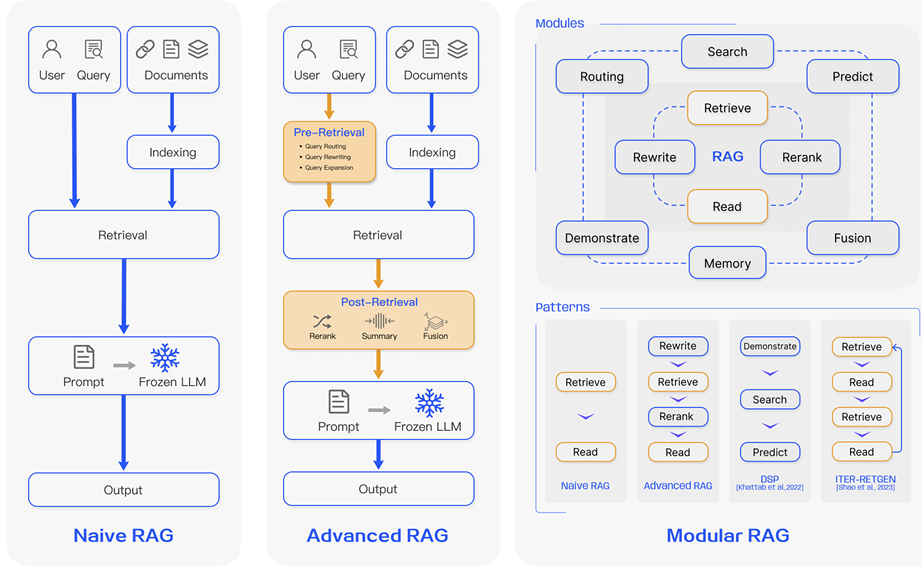
\includegraphics[width=0.9\linewidth]{Figures/rag_types.png}
	\caption{Types of RAG Systems}
	\label{rag_architectur.png}
\end{figure}
\subsection{Naive (RAG)}
Naive RAG, a foundational approach in Retrieval-Augmented Generation, operates on a straightforward "Retrieve-Read-Generate" paradigm. This method involves three primary steps:

\begin{itemize}
	\item Indexing: Raw data is cleaned, extracted, and converted into a uniform text format. It's then segmented into smaller chunks and encoded into vector representations using an embedding model. These vectors are stored in a vector database for efficient similarity searches.
	\item Retrieval: When a user query is received, it's encoded into a vector and compared to the indexed chunks. The top K most similar chunks are retrieved and included in the prompt for the language model.
	\item Generation: The query and retrieved chunks are combined into a prompt, which is fed to a large language model. The model generates a response based on the provided context and its internal knowledge.
\end{itemize}
While Naive RAG offers a basic framework, it faces several challenges in 
\begin{itemize}
	\item Retrieval Issues: The retrieval process can be imprecise, leading to the selection of irrelevant or missing information.
	\item Generation Challenges: The language model may hallucinate, generating content not supported by the retrieved context. It may also produce irrelevant, toxic, or biased outputs.
	\item Augmentation Difficulties: Integrating retrieved information into the generation process can be challenging, leading to disjointed or redundant responses.
\end{itemize}

\subsection{Advanced (RAG)}
Taking aim at the shortcomings of Naive RAG, Advanced RAG introduces specific improvements to enhance retrieval quality. This approach utilizes pre-retrieval and post-retrieval strategies.\\
\textbf{Pre-retrieval Strategies:}
\begin{itemize}
	\item Enhanced Indexing: Advanced RAG tackles indexing issues through a sliding window approach, finer segmentation of data, and inclusion of metadata. Additionally, it optimizes the retrieval process by employing various methods.
	\item Query Optimization: This stage focuses on refining the user's initial query to make it clearer and more suitable for retrieval. Techniques like query rewriting, transformation, and expansion are commonly used.
\end{itemize}
\textbf{Post-Retrieval Strategies:}
\begin{itemize}
	\item Re-ranking Chunks: After relevant information is retrieved, Advanced RAG prioritizes the most relevant content by re-ranking the retrieved chunks and placing them strategically within the prompt.
	\item Context Compression: To avoid overwhelming the LLM with too much information, post-retrieval efforts focus on selecting the most essential parts of the retrieved context, highlighting critical sections, and compressing the data to be processed.
\end{itemize}
By addressing indexing issues and refining the query and retrieved information, Advanced RAG aims to improve the overall accuracy and relevance of the generated response.
\subsection{Modular (RAG)} 
Modular RAG represents the latest evolution in RAG, offering greater adaptability. it introduces specialized modules and innovative patterns to enhance retrieval and processing capabilities.\\
\textbf{New Modules}
\begin{itemize}
	\item Search Module: Adapts to specific scenarios by leveraging LLM-generated code and query languages to search across various data sources.
	\item RAG Fusion: Employs a multi-query strategy to expand user queries, uncover both explicit and implicit knowledge, and improve retrieval results.
	\item Memory Module: Leverages the LLM's memory to guide retrieval and create an unbounded memory pool, aligning the text more closely with data distribution.
	\item Routing Module: Navigates through diverse data sources, selecting the optimal pathway for a query based on its specific needs.
	\item Predict Module: Reduces redundancy and noise by generating relevant context directly through the LLM.
	\item Task Adapter Module: Tailors RAG to various downstream tasks by automating prompt retrieval and creating task-specific retrievers.
\end{itemize}
\textbf{New Patterns} 
\begin{itemize}
	\item Flexible Module Arrangement: Modular RAG allows for the substitution and reconfiguration of modules to address specific challenges, surpassing the fixed structures of previous RAG paradigms.
	\item Innovative Retrieval Strategies: Techniques like Rewrite-Retrieve-Read, Generate-Read, and Recite-Read leverage the LLM's capabilities to refine queries, generate content, and retrieve information from model weights.
	\item Hybrid Retrieval: Combines keyword, semantic, and vector searches to cater to diverse queries, improving retrieval relevance.
	\item Dynamic Module Interaction: Frameworks like Demonstrate-Search-Predict and ITERRETGEN demonstrate the dynamic use of module outputs to enhance each other's functionality.
	\item Adaptive Retrieval: Techniques like FLARE and Self-RAG evaluate the necessity of retrieval based on different scenarios, allowing for a more flexible and efficient approach.
	
\end{itemize}
\section{Core Components of RAG}
The core components of Retrieval-Augmented Generation (RAG) systems consist of a retrieval mechanism, a generation process, and augmentation techniques. These elements work together to enhance the model's ability to access relevant external information, generate coherent and contextually appropriate responses, and improve overall performance in knowledge-intensive tasks.
\subsection{ Retrieval Mechanism}
RAG systems combine parametric memory (a pre-trained language model) with non-parametric memory (a retrieval mechanism). The retrieval mechanism allows RAG models to access external information sources (e.g., Wikipedia), and this process is central to improving the model's ability to generate factual and accurate outputs \cite{lewis2020retrieval}.
\begin{itemize}
	\item Traditional Techniques: \\
	Classical retrieval methods include \textbf{TF-IDF and BM25}, which rely on sparse vector representations based on term frequencies. These methods use exact keyword matching, making them limited in semantic understanding.
	\item Modern Retrieval Approaches:\\
	\textbf{ Dense Passage Retrieval (DPR): }This approach utilizes dense vector representations learned by neural models like BERT to encode both the query and document. It allows for a more semantic understanding of the content, making retrieval more effective. DPR, for example, computes the similarity between the query and documents using Maximum Inner Product Search (MIPS), which finds the closest passages based on the dense vector space.
	\item Implementation in RAG:\\ In RAG, dense retrieval methods are often paired with techniques like \textbf{Maximum Inner Product Search} (MIPS), which efficiently matches query and document embeddings. This enables the system to return the most relevant documents for subsequent generation \cite{karpukhin2020dense}.
	
\end{itemize}
\subsection{Generation Process}
The generation in RAG occurs through a combination of retrieved passages and the input query.\\
Large Language Models (LLMs) like BART or T5 are utilized for this generation, leveraging their advanced capabilities in understanding and producing human-like text. The retrieval component supplies external context, which the generator conditions on to formulate a response.This context is crucial, as it enriches the LLM's understanding, enabling it to incorporate real-time, relevant information. Moreover, the generation process benefits from the LLM's ability to synthesize information, allowing it to create responses that are not only coherent but also informed by the latest data, thus improving accuracy and relevance in knowledge-intensive tasks \cite{lewis2020retrieval}. \\
\begin{figure}[h]
	\centering
	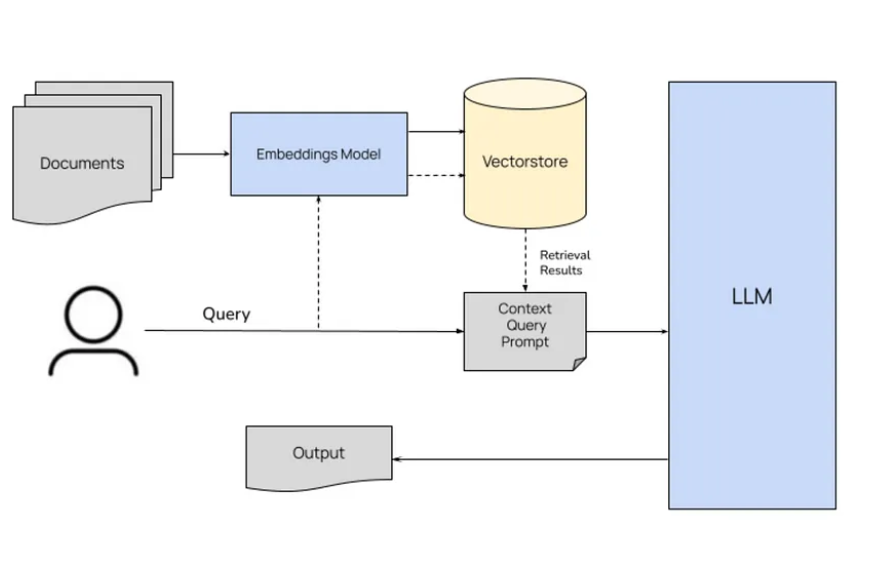
\includegraphics[width=0.9\linewidth]{Figures/rag_architectur.png}
	\caption{Rag architecture}
	\label{rag_architectur.png}
\end{figure}
\subsection{ Augmentation Techniques}
The augmentation of the retrieval process in Retrieval-Augmented Generation (RAG) systems focuses on improving how queries are refined and how relevant information is retrieved for downstream generation tasks. Key augmentation methods include.
\begin{itemize}
	\item \textbf{Query Augmentation:} In traditional retrieval pipelines, user queries are often under-specified or ambiguous, leading to poor retrieval performance. Query augmentation involves dynamically rewriting the user's query to better match the documents in the knowledge base. This can be done by leveraging large language models (LLMs) to generate tailored queries or synthetic questions and answers (QAs) that better align with the search objective​
	\item \textbf{Synthetic QA Generation:} Instead of using raw document chunks, retrieval is enhanced by generating and embedding synthetic QA pairs from documents. This helps to capture the semantic essence of long texts more effectively, reducing noise and improving retrieval precision. These synthetic QAs can be used to rewrite the user query, making it more specific to the task at hand \cite{mombaerts2024meta}.
\end{itemize}
\section{RAG for Legal Information Retrieval}

Retrieval-Augmented Generation (RAG) holds significant promise for transforming the way legal information is accessed, processed, and utilized. In legal contexts, particularly where precision and comprehensiveness are critical, RAG enables the dynamic integration of relevant external knowledge into language models during inference. This is especially valuable for retrieving and synthesizing content from case law, legislative texts, legal commentaries, and scholarly analyses\cite{lexemoRAG}.

Unlike traditional keyword-based or Boolean legal search systems, which rely on exact matches and rigid query structures, RAG models operate by embedding both queries and documents into a shared vector space, allowing for more semantic and contextual retrieval. This enables users to pose natural language queries and obtain responses grounded in specific, retrieved legal documents. For instance, rather than retrieving a list of documents containing the keyword "contract termination," a RAG model can retrieve multiple relevant legal provisions, judgments, or commentaries and synthesize a coherent and accurate summary or answer.

Moreover, RAG is well-suited to handle the diversity and complexity of legal texts. It can retrieve from multiple sources—statutes, judicial rulings, legal doctrines—and present consolidated outputs that reduce the time and effort needed for legal research. In contexts where laws are updated frequently or where legal reasoning requires multi-document understanding, such as in complex case analysis, RAG provides an efficient, scalable alternative to traditional systems.

The potential benefits are particularly evident when applied to under-resourced legal systems or multilingual environments, such as in Algeria, where legal texts exist in both Arabic and French, and digital legal resources remain fragmented. Here, RAG could offer a pathway toward more accessible, interpretable, and comprehensive legal information services\cite{asteraRAG}.


\section{Task and Evaluation}
The rapid development and increasing use of Retrieval-Augmented Generation (RAG) models in NLP have made their evaluation a critical area of research within the LLM community. This section covers the primary downstream tasks associated with RAG, the datasets used, and the methods for evaluating RAG systems \cite{zhou2020trustworthiness}.
\subsection{Factuality}
\begin{itemize}
	\item Fact-Checking Benchmarks: Using datasets like FEVER and SQuAD to evaluate the model's ability to identify and correct factual errors.
	\item Adversarial Testing: Creating adversarial examples to test the model's robustness against misleading information.
	\item Contextual Understanding: Assessing the model's ability to understand the context of a query and provide accurate answers.
\end{itemize}
\subsection{ Robustness}
\begin{itemize}
	\item Noise Injection: Introducing noise into the retrieved documents to test the model's ability to handle imperfect information.
	\item Adversarial Attacks: Evaluating the model's resilience to attacks that aim to manipulate its outputs.
	\item Domain Adaptation: Testing the model's ability to adapt to new domains and data distributions.
\end{itemize}
\subsection{Fairness}
\begin{itemize}
	
	\item Bias Detection: Identifying and quantifying biases in the training data and model outputs.
	\item Fairness Metrics: Using metrics like demographic parity and equalized odds to evaluate the model's fairness.
	\item Mitigation Techniques: Implementing techniques like debiasing and fairness constraints to mitigate biases.
\end{itemize}
\subsection{Objective Metrics:}
\begin{itemize}
	\item Accuracy: Precision, recall, and F1-score for evaluating the correctness of the generated responses.
	\item Consistency: Measuring the consistency of the model's outputs across different queries and contexts.
	\item Coherence: Assessing the coherence and fluency of the generated text.
\end{itemize}
\subsection{Subjective Metrics}
\begin{itemize}
	\item Human Evaluation: Using human raters to evaluate the quality of the generated responses.
	\item User Studies: Conducting user studies to gather feedback on the user experience
\end{itemize}
\section{ Challenges and Limitations in (RAG)}
While RAG has gained significant traction across diverse applications, it still faces certain limitations in terms of effectiveness and efficiency\cite{zhao2024retrieval} \cite{gupta2024comprehensive}.
\subsection{Scalability and Efficiency}
A major challenge for RAG models lies in their scalability. Since retrieval components depend on external databases, efficiently handling large and constantly expanding datasets demands robust retrieval algorithms. Additionally, the high computational and memory requirements pose difficulties for deploying RAG models in real-time or resource-limited environments
\subsection{Noisy Retrieval Results}
The quality of retrieval results can significantly impact the performance of Retrieval-Augmented Generation (RAG) models. Several factors contribute to noisy retrieval, including the methods used for indexing, the way queries are formulated, and the characteristics of the underlying datasets. When irrelevant or noisy information is retrieved, it may result in the generation of hallucinated or factually inaccurate responses, further compromising the reliability of the system. Additionally, the model’s ability to correctly interpret the retrieved information can be hindered, particularly when the information lacks proper formatting or contains inconsistencies. 
\subsection{Bias and Fairness} 
Like other machine learning models, Retrieval-Augmented Generation (RAG) systems can inherit biases from the datasets they rely on for retrieval. These biases may be amplified during the generation process, potentially leading to biased or harmful outputs. Addressing this issue by developing effective techniques to mitigate bias in both the retrieval and generation phases remains an ongoing challenge.
\subsection{Extra Overhead}
\begin{itemize}
	\item Computational Cost: Retrieval and processing additional information can increase computational costs, especially for large-scale models and complex queries.
	\item Latency: Retrieval and processing can introduce latency, impacting the real-time performance of RAG systems.
	\item Complexity: Implementing and deploying RAG systems requires careful consideration of various factors, including data preparation, model selection, and system architecture.
\end{itemize}

\subsection{Long Context Generation:}

\begin{itemize}
	\item Context Length Limits: LLMs have limitations on the amount of context they can process at once.
	\item Information Loss: Long documents may be truncated or summarized, leading to loss of important information.
	\item Computational Cost: Processing long contexts can be computationally expensive.
\end{itemize}
\newpage
\section{Conclusion}


In this chapter, we explored the core principles and mechanisms of Retrieval-Augmented Generation (RAG), emphasizing its potential to enhance language models through access to external knowledge sources during inference. We examined its general architecture, key stages, and its evolution from naive to more modular frameworks. 

A particular focus was placed on the application of RAG in the legal domain, where we highlighted its potential for improving legal information retrieval by enabling more contextualized and semantically rich access to case law, statutes, and scholarly texts. We also outlined the main challenges and limitations facing RAG models, including noisy retrieval, bias, scalability.

Following this foundational understanding, the next chapter delves into a critical aspect of RAG performance: the problem of knowledge selection. Specifically, we explore how the effectiveness of retrieved documents directly influences the quality of generated responses, and we investigate strategies to improve relevance and ranking within RAG pipelines.
